\documentclass[12pt]{article}
\usepackage[margin=1in]{geometry}
\usepackage{graphicx}
\usepackage{amsmath}
\usepackage{tikz}

\newcommand{\comment}[1]{}
\newcommand{\ihat}{\hat{\textbf{\i}}}
\newcommand{\jhat}{\hat{\textbf{\j}}}

\title{What the hell is a linear combination?}
\author{}
\date{}

\begin{document}
\maketitle

\section{A (yet another) different way to think about vectors}
Well consider a 2D co-ordinate system. Say we draw the vector $ \comment{Column-Vector: 2, -3} \begin{pmatrix} 2 \\  -3 \end{pmatrix} $ in that system.

\begin{figure}[h]
  \centering
  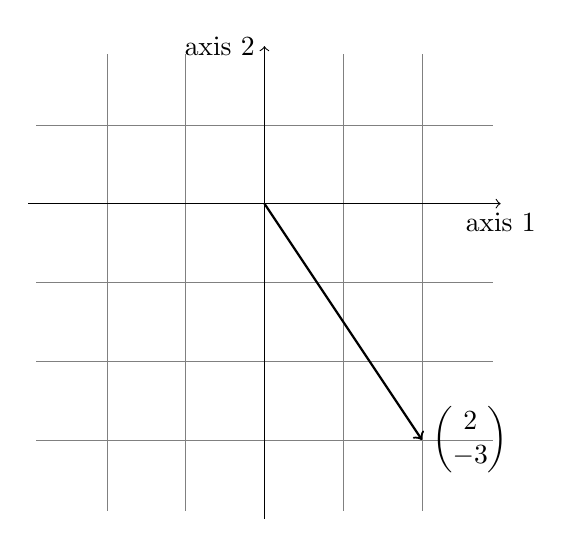
\begin{tikzpicture}
    \draw[step=1cm,gray,very thin] (-2.9,-3.9) grid (2.9,1.9);
    \draw[->] (-3, 0) -- (3, 0) node[anchor=north] {axis 1};
    \draw[->] (0, -4) -- (0, 2) node[anchor=east] {axis 2};
    \draw[thick, ->] (0, 0) -- (2, -3) node[anchor=west] { $ \comment{Column-Vector: 2, -3} \begin{pmatrix} 2 \\  -3 \end{pmatrix} $  };
  \end{tikzpicture}
\end{figure}

We know that each number in the list (the vector) is the signed length that we need to travel to get to the point represented by the vector.
Well we can also `think' that \textbf{each number represents the `scalar' that scales some very fundamental vectors that belong to the system and by adding the scaled versions of those vectors we get the same point}.

This idea of \textbf{scaling and adding things is known as linear combination} in general. In linear algebra the things are vectors. Most ideas in linear algebra build up on this idea of scaling and adding some fundamental vectors (i.e. linear combination of vectors). In the regular 2D co-ordinate system these vectors are $ \ihat $ and $ \jhat $.

So a linear combination of $ \ihat $ and $ \jhat $ can be represented symbolically as \[
\alpha * \ihat + \beta * \jhat
.\] where $ \alpha $ and $ \beta $ are any real numbers.

The word comes from I guess the fact that there are other types of combinations like polynomial combination, exponential combination, logarithmic combination and what not. The most simplest of them all for us humans seems to be linear combination. And we know from experience that simple is fun and often powerful.

\end{document}
